\newsection{Processi primari}
\subsection{Fornitura}
Il fine di questa sezione è definire le norme che i membri del gruppo 7DOS sono invitati a rispettare con l'obiettivo di proporsi e diventare fornitori nei confronti dell'azienda proponente Zucchetti s.r.l. e dei committenti Prof. Tullio Vardanega e Prof. Riccardo Cardin per quanto concerne il prodotto \emph{G\&B}.
Per raggiungere questa meta nel miglior modo possibile, abbiamo intenzione di collaborare in modo \gl{efficiente} e \gl{efficace} con i referenti dell'azienda.
I punti fondamentali che verranno affrontati insieme al proponente saranno:
\begin{itemize}
\item Determinare gli aspetti cruciali al fine di soddisfare l'azienda proponente;
\item Concordare la qualifica del prodotto;
\item Determinare vincoli sui processi e sui requisiti;
\item Stimare i costi del prodotto finale.
\end{itemize}
Di seguito sono riportate tutte le attività che compongono questo processo:

\subsubsection{Attività}

\paragraph{Studio del dominio tecnologico} \Spazio
Consiste nella ricerca di tutte quelle informazioni relative alle tecnologie e nella valutazione di possibili alternative utili al fine del progetto. Ne consegue che i risultati ottenuti, frutto di informazioni reperite ed esperienze personali, devono prima essere discussi, approvati ed eventualmente concordati con la proponente.
Ogni componente del gruppo è incaricato di approfondire o studiare autonomamente le tecnologie necessarie allo sviluppo del progetto, in modo da ottenere buona padronanza del dominio tecnologico impiegato.

\paragraph{Normazione} \Spazio
La definizione delle norme potrebbe subire delle variazioni con il progredire del progetto; ciò è dovuto a nuove necessità a cui il gruppo andrà incontro ed eventuali problematiche che potrebbero essere riscontrate. Sarà quindi \gl{compito} degli \emph{Amministratori} sopperire a queste complicazioni redigendo nuove norme o modificando quelle già presenti.

\paragraph{Studio di Fattibilità} \Spazio
Nel documento \emph{Studio di Fattibilità v1.0.0.} troviamo le motivazioni che hanno portato il nostro gruppo a favorire la scelta del prodotto per cui proporci come fornitori. Inoltre, si riportano, per ogni capitolato, le seguenti informazioni:
\begin{itemize}
 	\item\textbf{{Descrizione}}: riporta una breve sintesi del prodotto da sviluppare;
 	\item\textbf{{Studio del dominio}}: riporta un'analisi del dominio applicativo, in cui vi è una più corposa descrizione del prodotto da sviluppare con l'aggiunta di una generale contestualizzazione, e un'analisi del dominio tecnologico, in cui vengono elencate le maggiori tecnologie coinvolte per ogni prodotto secondo la descrizione del capitolato e dalle esperienze pregresse dei componenti del gruppo;
 	\item\textbf{{Valutazione generale}}: composta dagli aspetti positivi e dagli aspetti negativi trovati e discussi dal gruppo riguardo al capitolato in esame;
 	\item\textbf{{Valutazione finale}}: vi si può trovare in breve la motivazione della scelta presa per ogni capitolato in base a ciò che è stato riportato nelle tre sezioni precedenti.
\end{itemize}

\paragraph{Pianificazione} \Spazio
Questa sezione descrive le attività per consegnare il
sistema al richiedente, rispettando dei vincoli imposti. Viene descritto un piano per analizzare e gestire i rischi di progetto, un budget di progetto, le attività da svolgere rispettando delle scadenze temporali definite e le convenzioni per revisionare le specifiche e testarle.
\subparagraph{Piano di Progetto} \Spazio
La redazione di un \gl{piano} da seguire durante la realizzazione del progetto spetta al \emph{Responsabile}, aiutato nelle scelte dagli \emph{Amministratori}. Il documento dovrà coprire le seguenti tematiche:
 \begin{itemize}
 	\item\textbf{{Analisi dei rischi}}: riporta una dettagliata analisi dei rischi che si potrebbero incontrare durante la realizzazione del progetto, determinandone, in base alle conoscenze pregresse e alle nuove acquisite, la probabilità che essi accadano e la loro gravità. Inoltre, quando possibile, verranno analizzati i possibili metodi per affrontarli;
 	\item\textbf{{Pianificazione}}: viene presentata una pianificazione delle \gl{attività} da svolgere nel corso del progetto, fornendo delle scadenze temporali il più possibile precise e veritiere;
 	\item {\textbf{Assegnazione risorse}: riporta la suddivisione oraria delle risorse, tenendo conto dei ruoli ricoperti da tutti i membri. In questo modo si ha una visione chiara su come il gruppo sta procedendo e quante ore vengono impiegate per ogni attività;}
 	\item\textbf{{Preventivo}}: sulla base della pianificazione, viene stimata la quantità di lavoro necessaria per portare a termine ogni attività (e quindi ogni fase) del progetto, per arrivare infine ad avere una valutazione complessiva per tutto il progetto e proporre un preventivo finale con il costo del lavoro precedentemente stimato.
 \end{itemize}

Gli strumenti di supporto da utilizzare sono:
\begin{itemize}
	\item \textbf{Gantt Project}: per quanto riguarda la creazione dei diagrammi di Gantt abbiamo deciso di utilizzare Gantt Project data la sua completezza, facilità di utilizzo e la possibilità di esportare i diagrammi sotto forma di \gl{PNG}. Inoltre, i file di Gantt Project sono salvati in formato \gl{XML}, quindi facilmente versionabili;
	\item \textbf{Microsoft Excel}: per la realizzazione dei consuntivi abbiamo deciso di utilizzare Microsoft Excel come strumento per creare i grafici, data la sua efficacia e facilità di utilizzo.
\end{itemize}

\subparagraph{Piano di Qualifica} \Spazio
Il compito di \gl{verifica} e \gl{validazione} viene svolto da parte dei \emph{Verificatori}. Questa mansione verrà svolta secondo un preciso metodo che deve coprire le seguenti tematiche:
\begin{itemize}
	\item\textbf{{Metodo di verifica}}: riporta le procedure di controllo sulla \gl{qualità} di \gl{processo} e di \gl{prodotto}, considerando i mezzi e le risorse a disposizione;
	\item\textbf{{Misure e metriche}}: presenta criteri oggettivi per i documenti, i processi e il software;
	\item\textbf{{Gestione della revisione}}: precisa nel dettaglio le metodologie di comunicazione delle procedure di controllo per la qualità di processo e delle anomalie;
	\item\textbf{{Pianificazione del collaudo}}: definisce dettagliatamente le metodologie di collaudo a cui sarà sottoposto il progetto realizzato;
	\item\textbf{{Resoconto dell'attività di verifica}}: riporta le metriche calcolate e il resoconto sul collaudo delle attività sottoposte a verifica e validazione.
\end{itemize}


\paragraph{Ingresso alle revisioni} \Spazio
Prima di ogni revisione è fondamentale allestire ed organizzare correttamente il materiale da consegnare. Compito del \emph{Responsabile di Progetto} è redigere la lettera di presentazione da includere anch'essa per l'ingresso alla revisione.

\subsection{Sviluppo}
Il processo in questione affronta le attività ed i compiti svolti dal gruppo con l'obiettivo di sviluppare il software richiesto dal proponente. Per una corretta implementazione è fondamentale:
\begin{itemize}
		\item Realizzare un prodotto finale conforme alle richieste del proponente;
		\item Realizzare un prodotto finale che soddisfa i test di verifica e validazione;
		\item Fissare gli obiettivi di sviluppo;
		\item Fissare i vincoli tecnologici e di design.
\end{itemize}
Inoltre, il gruppo ha deciso di seguire le linee guida dettate dallo standard \gl{ISO}/\gl{IEC} 12207. Per questo motivo le attività scelte alla base del progetto di sviluppo saranno le seguenti:
\begin{itemize}
	\item Analisi dei Requisiti;
	\item Progettazione;
	\item Codifica.
\end{itemize}
\subsubsection{Analisi dei requisiti}
\paragraph{Scopo}\Spazio
Determinare con precisione i requisiti del progetto ed elencarli in modo formale. Essi vengono estrapolati da varie fonti:
\begin{itemize}
	\item Documenti di specifica del \gl{capitolato};
	\item Incontri con l'azienda proponente;
	\item Verbali interni ed esterni;
	\item Casi d'uso.
\end{itemize}
\paragraph{Casi d'uso}\Spazio
Ogni caso d'uso è descritto dalla seguente struttura:
\begin{itemize}
	\item Codice identificativo: $$ \textbf{UC \{codice\_padre\}.\{codice\_figlio\}  } $$
		\begin{itemize}
				\item UC specifica che si tratta di un caso d'uso;
				\item Codice\_padre identifica univocamente i casi d'uso;
				\item Codice\_figlio è un numero progressivo che identifica i sottocasi.
		\end{itemize}
	\item Titolo;
	\item Diagramma UML;
	\item Attori;
	\item Attori secondari (se presenti);
	\item Scopo e descrizione;
	\item Precondizione;
	\item Scenario principale;
	\item Postcondizioni;
	\item Inclusioni (se presenti);
	\item Estensioni (se presenti).
\end{itemize}
\paragraph{Requisiti}\Spazio
Ogni requisito è descritto dalla seguente struttura:
\begin{itemize}
	\item Nome;
	\item Tipo;
	\item Importanza;
	\item Stato implementazione;
	\item Fonti.
\end{itemize}

Inoltre, a ciascun requisito corrisponde un codice identificativo cosi composto:
$$ \textbf{R \{importanza\}.\{tipo\}.\{identificativo\}  } $$
\begin{itemize}
	\item R specifica che si tratta di un requisito ;
	\item Importanza identifica la rilevanza del requisito e può assumere 3 valori:
	\begin{itemize}
		\item 0: indica che il requisito è obbligatorio e il suo soddisfacimento dovrà necessariamente avvenire;
		\item 1: indica che il requisito è desiderabile, cioè il suo soddisfacimento può portare maggiore completezza al sistema ma non è fondamentale per lo stesso;
		\item 2: indica che il requisito è opzionale, e quindi la decisione di implementarlo o meno verrà presa dopo le dovute considerazioni;
	\end{itemize}
	\item Tipo distingue se si tratta di un requisito funzionale (F), di qualità (Q), di prestazione (P) o di vincolo (V);
	\item Identificativo è un numero progressivo che identifica i sottocasi.
\end{itemize}
\paragraph{UML}\Spazio
I diagrammi UML devono essere realizzati usando la versione del linguaggio \emph{v2.0}
\paragraph{Strumenti di supporto}
\subparagraph{Trender}\Spazio
Per quanto riguarda il tracciamento dei requisiti, il gruppo ha deciso di utilizzare inizialmente uno strumento non totalmente adatto a questo compito, cioè un foglio di calcolo. Essendo a conoscenza delle limitate funzionalità offerte da questa tecnologia per lo scopo a noi d'interesse, il team 7DOS ha deciso di migrare i dati raccolti in uno strumento creato appositamente per questo scopo. Lo strumento scelto è Trender e rende il tracciamento dei requisiti semi-automatico, inoltre offre la creazione di file .tex per il tracciamento dei requisiti.
\subparagraph{Astah UML}\Spazio
Per quanto concerne la creazione e la modellazione dei diagrammi UML per i casi d'uso, abbiamo deciso di utilizzare Astah UML, data la sua facilità di utilizzo e compatibilità con UML 2.0. Per la successiva fase di modellazione delle classi, potrebbe verificarsi una scelta diversa riguardo al software da utilizzare.
\subsubsection{Progettazione}
La presente sezione sarà soggetta ad incrementi durante la fase di "Progettazione di dettaglio e codifica". Per questo motivo, non si pone l'obiettivo di risultare completa in questa fase del progetto.
\paragraph{Scopo}\Spazio
La Progettazione esplicita concretamente una prima forma ad alto livello del design del software pensata per il progetto, determinandone le caratteristiche più in evidenza, in modo da comunicare con gli stakeholder e dare delle informazioni chiare, così da intraprendere le prime discussioni sul progetto. I \emph{Progettisti} hanno il compito di definire il sistema in modo esplicito così da poter fare importanti considerazioni riguardo a performance, affidabilità e manutenibilità, capire come è organizzato il sistema  e come i componenti interoperano tra di loro sottolineando la possibilità di riutilizzo in larga scala di parte del codice, dato che abbiamo notato una frequente ripetizione dei requisiti in un sistema complesso come quello affrontato dal nostro team.
L’architettura dovrà avere le seguenti caratteristiche:
	\begin{itemize}
		\item \textbf{Sufficienza}: deve essere in grado di soddisfare i requisiti decritti nel documento \emph{Analisi dei Requisiti};
		\item \textbf{Comprensibilità}: deve essere capita dagli stakeholder;
		\item \textbf{Flessibilità}: deve permettere modifiche in seguito a delle variazioni, senza essere profondamente ristrutturata;
		\item \textbf{Modularità}: deve essere composta di parti chiare e ben definite;
		\item \textbf{Riusabilità}: le parti devono poter essere usate in più applicazioni;
		\item \textbf{Efficienza}: deve ridurre al minimo gli sprechi;
		\item \textbf{Affidabilità}: deve rispettare le specifiche nel tempo;
		\item \textbf{Disponibilità}: non deve essere inabilitata durante la manutenzione;
		\item \textbf{Sicurezza}: non deve essere vulnerabile ad intrusioni e malfunzionamenti;
		\item \textbf{Semplicità}: deve contenere solo il necessario;
		\item \textbf{Incapsulazione}: le informazioni interne delle componenti devono essere nascoste;
		\item \textbf{Coesione}: le parti che condividono lo stesso fine devono stare insieme;
		\item \textbf{Basso accoppiamento}: parti diverse devono essere poco dipendenti dalle altre.
	\end{itemize}
\paragraph{Attività}\Spazio
Il design del software non è composto da una singola attività, bensì da un insieme preciso di sotto-attività progettuali che portano al design finale.
Le sotto-attività che il nostro gruppo ha scelto di svolgere sono:
	\begin{itemize}
	\item\textbf{{Progettazione architetturale}}: i progettisti identificheranno una struttura globale del sistema, quindi i componenti principali, le loro relazioni e come saranno distribuiti;
	\item\textbf{{Progettazione dell'interfaccia}}: i progettisti definiranno le interfacce tra i \gl{moduli} di sistema. Ciò deve essere fatto assolutamente in modo non ambiguo dato che, grazie a queste specifiche, ogni componente potrà usare in modo appropriato le funzionalità degli altri componenti del progetto senza sapere l'effettiva implementazione;
	\item\textbf{{Selezione e progettazione dei componenti}}: i progettisti cercheranno dei componenti riutilizzabili e valuteranno se inserirli nel progetto, specificandone gli appropriati utilizzi e aggiustamenti, o se sarà più opportuno costruire dei nuovi componenti.
\end{itemize}
\paragraph{Diagrammi}\Spazio
Per rendere più chiare le scelte progettuali adottate e ridurre le possibili ambiguità, verranno impiegate le seguenti tipologie di rappresentazioni:
\begin{itemize}
	\item \textbf{Diagrammi delle classi}: per descrivere gli oggetti presenti nel sistema;
	\item \textbf{Diagrammi dei package}: per descrivere le dipendenze delle classi raggruppate in package;
	\item \textbf{Diagrammi di sequenza}: per descrivere la collaborazione nel tempo tra un gruppo di oggetti;
	\item \textbf{Diagrammi di attività}: per descrivere la logica procedurale.
\end{itemize}
\paragraph{Diagrammi delle classi}\Spazio
Lo scopo dei diagrammi delle classi è:
\begin{itemize}
	\item Fornire la progettazione della visione statica di un'applicazione;
	\item Descrivere le responsabilità di un sistema;
	\item Base per diagrammi dei componenti e di rilascio;
	\item \gl{Reverse Engineering}.
\end{itemize}
I diagrammi delle classi sono collegati fra loro da frecce che ne esplicitano le dipendenze. \\
Verranno utilizzati i seguenti tipi di freccia:
\begin{itemize}

\item Indica che la classe A ha fra i propri campi dati una o più istanze della classe B;
\begin{figure} [H]
	\centering
	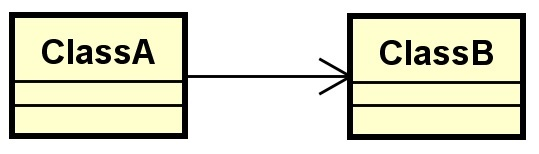
\includegraphics[scale=0.75]{./Img/dipendenza_forte.jpg}
	\caption{Relazione di dipendenza forte tra classi}\label{}
\end{figure}

\item  Indica che A dipende da B secondo una primitiva;
\begin{figure} [H]
	\centering
	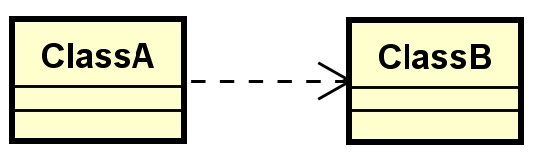
\includegraphics[scale=0.75]{./Img/dipendenza.jpg}
	\caption{Relazione di dipendenza debole tra classi}\label{}
\end{figure}

\item Indica un'aggregazione da A verso B, cioè una relazione non forte nella quale le classi parte hanno un significato anche senza che sia presente la classe tutto;
\begin{figure} [H]
	\centering
	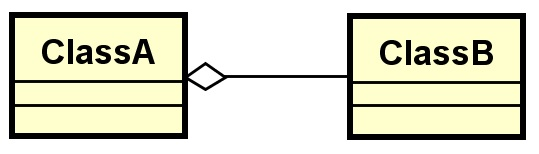
\includegraphics[scale=0.75]{./Img/aggregazione.jpg}
	\caption{Relazione di aggregazione tra classi}\label{}
\end{figure}

\item Indica una composizione da A verso B, cioè una relazione forte nella quale le classi parte hanno un reale significato solo se sono legate alla classe tutto;
\begin{figure} [H]
	\centering
	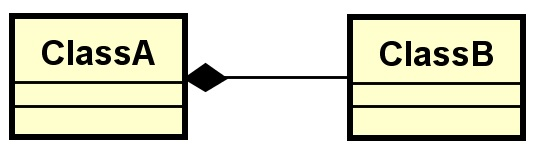
\includegraphics[scale=0.75]{./Img/composizione.jpg}
	\caption{Relazione di composizione tra classi}\label{}
\end{figure}

\item Indica l’ereditarietà, cioè che ogni oggetto di A è anche un oggetto di B.
\begin{figure} [H]
	\centering
	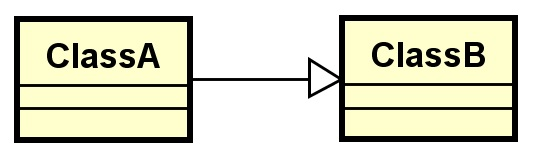
\includegraphics[scale=0.75]{./Img/ereditarieta.jpg}
	\caption{Relazione di ereditarietà tra classi}\label{}
\end{figure}

\end{itemize}

\paragraph{Diagrammi dei package}\Spazio
I package sono rappresentati in forma di rettangoli e dispongono di un nome univoco. Ogni rettangolo contiene i diagrammi delle classi presenti all'interno di quel package. Le dipendenze sono indicate da frecce tratteggiate.
Nel seguente esempio si può vedere che il package A ha una dipendenza nei confronti di B.
\begin{figure} [H]
	\centering
	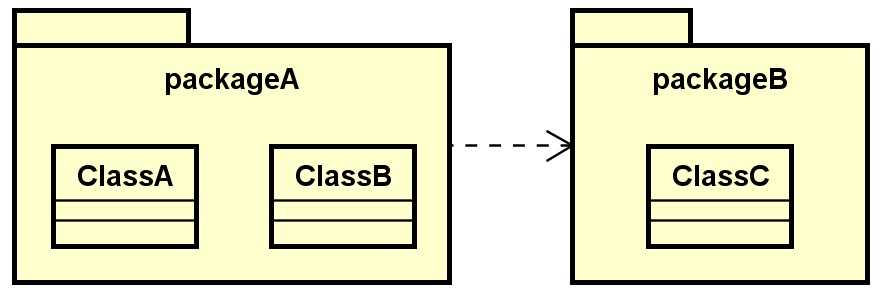
\includegraphics[scale=0.7]{./Img/package.jpg}
	\caption{Relazione di dipendenza tra package}\label{}
\end{figure}

\paragraph{Diagrammi di sequenza}\Spazio
Questi diagrammi hanno un verso di lettura dall'alto verso il basso, che indica lo scorrere del tempo. 
Gli oggetti presenti nei diagrammi di sequenza sono rappresentati da rettangoli, al cui interno è presente un nome per identificarli. Sotto ad ogni istanza è presente una linea tratteggiata verticale, che indica la vita dell'oggetto. Da esse possono partire o arrivare delle frecce orizzontali di attivazione, che si distinguono nelle seguenti tipologie:
\begin{itemize}
	\item Messaggi sincroni, in cui il chiamante resta in attesa di una risposta
	\begin{figure} [H]
		\centering
		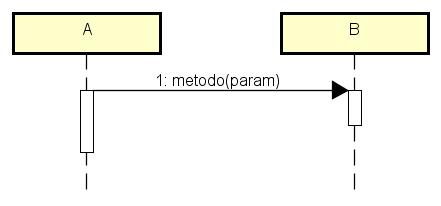
\includegraphics[scale=0.7]{./Img/sequence_sincrono.jpg}
		\caption{Messaggio sincrono}\label{}
	\end{figure}
	\item Messaggi asincroni, in cui il chiamante non rimane in attesa di una risposta
	\begin{figure} [H]
		\centering
		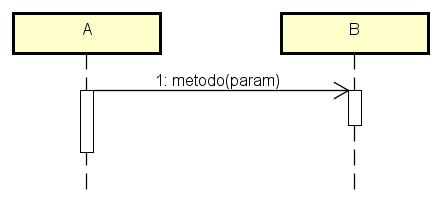
\includegraphics[scale=0.7]{./Img/sequence_asincrono.jpg}
		\caption{Messaggio asincrono}\label{}
	\end{figure}
	\item Messaggio di ritorno
	\begin{figure} [H]
		\centering
		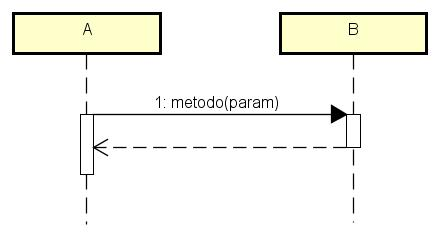
\includegraphics[scale=0.7]{./Img/sequence_ritorno.jpg}
		\caption{Messaggio di ritorno}\label{}
	\end{figure}
	\item Creazione e distruzione di un partecipante
	\begin{figure} [H]
		\centering
		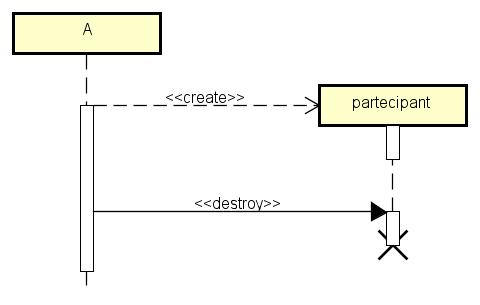
\includegraphics[scale=0.7]{./Img/sequence_partecipant.jpg}
		\caption{Messaggio di ritorno}\label{}
	\end{figure}
\end{itemize}

\paragraph{Diagrammi di attività}\Spazio
I diagrammi di attività aiutano a descrivere gli aspetti dinamici dei casi d'uso e supportano l'elaborazione parallela. Ogni attività viene rappresentata da un rettangolo dagli angoli arrotondati e contiene al suo interno il nome. Un diagramma si compone delle seguenti parti:
\begin{itemize}
	\item Nodo iniziale da dove inizia l'esecuzione del processo
	\begin{figure} [H]
		\centering
		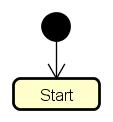
\includegraphics[scale=0.8]{./Img/attivita_start.jpg}
		\caption{Nodo iniziale}\label{}
	\end{figure}
	\item Fork per l'elaborazione parallela
	\begin{figure} [H]
		\centering
		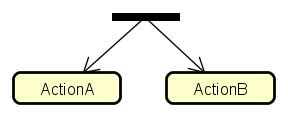
\includegraphics[scale=0.8]{./Img/attivita_fork.jpg}
		\caption{Fork di attività}\label{}
	\end{figure}
	\item Join per la sincronizzazione dei processi paralleli
	\begin{figure} [H]
		\centering
		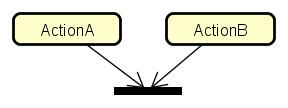
\includegraphics[scale=0.8]{./Img/attivita_join.jpg}
		\caption{Join dei processi paralleli}\label{}
	\end{figure}
	\item Branch per la scelta di uno dei rami decisionali
	\begin{figure} [H]
		\centering
		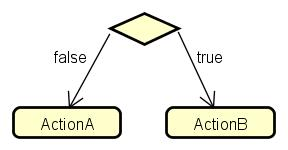
\includegraphics[scale=0.8]{./Img/attivita_branch.jpg}
		\caption{Branch per decisione}\label{}
	\end{figure}
	\item Merge per unire i rami separati dal branch
	\begin{figure} [H]
		\centering
		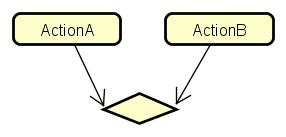
\includegraphics[scale=0.8]{./Img/attivita_merge.jpg}
		\caption{Merge per unire rami separati da branch}\label{}
	\end{figure}
	\item I segnali seguono la notazione seguente per indicare il tempo da aspettare prima dell'invio di un segnale, l'invio di un segnale e la sua ricezione
	\begin{figure} [H]
		\centering
		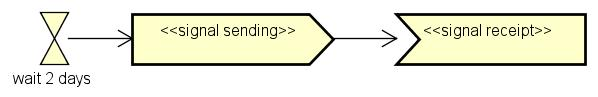
\includegraphics[scale=0.7]{./Img/attivita_segnali.jpg}
		\caption{Notazioni dei segnali}\label{}
	\end{figure}
	\item Nodo di fine flusso per indicare la terminazione di un ramo
	\begin{figure} [H]
		\centering
		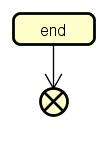
\includegraphics[scale=0.8]{./Img/attivita_fineflusso.jpg}
		\caption{Nodo di fine flusso}\label{}
	\end{figure}
	\item Nodo finale per indicare la terminazione dell'esecuzione
	\begin{figure} [H]
		\centering
		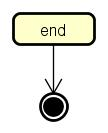
\includegraphics[scale=0.8]{./Img/attivita_fine.jpg}
		\caption{Nodo finale}\label{}
	\end{figure}
	
\end{itemize}

\paragraph{Tecnologie}\Spazio
Lo sviluppo del progetto richiede l'utilizzo di tecnologie, alcune imposte del capitolato, altre soggette a libera scelta da parte del team.
Le tecnologie il cui uso è obbligatorio sono:
\begin{itemize}
\item\textbf{{Grafana;}}
\item\textbf{{AngularJS;}}
\item\textbf{{InfluxDB.}}
\end{itemize}
Le tecnologie che invece il team ha scelto a valle di un attività di comparazione sono:
\begin{itemize}
\item\textbf{{TypeScript}}: per la scrittura del plug-in per Grafana;
\item\textbf{{Webpack}}: per il processo di build del plug-in;
\item\textbf{{JsBayes}}: per il calcolo delle probabilità delle reti Bayesiane;
\item\textbf{{NodeJS}}: per l'esecuzione lato server di codice JavaScript.
\end{itemize}
\paragraph{Integrazione continua}\Spazio
Il team ha scelto di applicare pratiche di integrazione continua e per farlo ha scelto di usare \gl{TravisCI}.
TravisCI è una piattaforma che permette di associare un repository GitHub ad un processo di build e ad un set di test di unità.
Ad ogni commit viene eseguito il processo di build e vengono eseguiti i test. TravisCI inoltre offre integrazione con \gl{Coveralls} un
servizio per la gestione del test coverage.
\subsubsection{Codifica}
La seguente sotto-sezione ha lo scopo di elencare le norme di codifica alle quali i Programmatori devono aderire durante l'attività di programmazione. Gli argomenti trattati riguardano:
\begin{itemize}
 \item{Norme generali dello stile di codifica da adottare, qualsiasi sia il linguaggio utilizzato;}
 \item{Norme specifiche per i linguaggi \gl{JavaScript,} \gl{TypeScript,} \gl{HTML} e \gl{CSS}.}
\end{itemize}
Il gruppo 7DOS ha deciso di porre delle norme sulla codifica in quanto vantaggiose per la generazione di codice leggibile, adatto per le fasi di verifica e manutenzione, e per garantire qualità al prodotto.
Soltanto il \emph{Responsabile di Progetto}, dopo un'attenta analisi e valutazione, potrà ammettere modifiche alle convenzioni stabilite.\\
\paragraph{Norme sul codice}
\begin{itemize}
	\item \textbf{Nomi}: i nomi di variabili, classi, funzioni e metodi dovranno essere in \gl{camel case} ed in lingua inglese. I nomi di variabili, metodi e funzioni dovranno avere la prima lettera minuscola mentre i nomi delle classi dovranno avere la prima lettera maiuscola.\\ Ogni nome deve essere unico e illustrativo, cioè deve richiamare lo scopo per cui è stato dichiarato.
	\item \textbf{Ricorsione}: la ricorsione va evitata quando possibile. Per ogni funzione ricorsiva sarà necessario fornire una prova di terminazione e sarà necessario valutare il costo in termini di occupazione della memoria. Nel caso l’utilizzo di memoria risulti troppo elevato la ricorsione verrà rimossa;
	\item \textbf{Intestazioni} \Spazio
	Ogni file contenente codice deve essere provvisto di un'intestazione contenente:

	\code{/*} \\
	\code{@File: nome del file} \\
	\code{@Version: versione del file} \\
	\code{@Type: tipo del file} \\
	\code{@Author: autore} \\
	\code{@Email: indirizzo email dell'autore} \\
	\code{@Date: data di creazione} \\
	\code{@Desc: descrizione del file}\\\\
	\code{@Changelog: autore, data, descrizione}\\
	\code{*/} \\

Ogni classe deve essere provvista di un'intestazione contenente:

	\code{/*} \\
	\code{@Class: nome della classe} \\
	\code{@Desc: descrizione della classe} \\
	\code{*/}\\

Ogni funzione e metodo devono essere provvisti di un'intestazione contenente:

	\code{/*} \\
	\code{@Desc: descrizione della funzione/metodo} \\
	\code{@Param: elenco dei parametri} \\
	\code{@Return: valore ritornato} \\
	\code{*/}\\

	\item \textbf{Commenti}: i commenti devono essere esaustivi e non prolissi in modo da aiutare il lettore a comprendere al meglio ciò che si sta leggendo. I commenti devono essere scritti in inglese. Inoltre è consentito l'uso di particolari tipi di commenti che hanno l'obiettivo di favorire la stesura del codice come:
	\begin{itemize}
		\item TODO: per segnalare la presenza di funzionalità che devono ancora essere implementate;
		\item FIX: per segnalare la presenza di un errori che devono ancora essere corretti.
	\end{itemize}

	\item \textbf{Versionamento:} la versione del file, inserita all'interno dell'intestazione, segue la convenzione \textbf{X.Y}.
	\begin{itemize}
		\item{\textbf{X}: indica l'indice di versione principale. Incrementare il suo valore indica che sono state apportate modifiche significative e stabili al file, comportando di conseguenza l'azzeramento dell'indice Y;}
		\item{\textbf{Y}: indica l'indice di versione parziale. Incrementare il suo valore indica che sono state apportate modifiche minori, come l'aggiunta o la rimozione di un metodo.}
	\end{itemize}
	Entrambe gli indici partono da 0. La versione \emph{1.0} indica la prima versione stabile del file, la quale copre le funzionalità obbligatorie.
\end{itemize}

\paragraph{JavaScript}\Spazio
Le convenzioni stilistiche definite in \gl{JavaScript Style Guide and Coding Conventions}\footnote{\url{https://www.w3schools.com/js/js_conventions.asp}} verranno seguite dai \emph{Programmatori} per lo sviluppo dell'intero progetto.

\begin{itemize}
	\item{\textbf{Indentazione}}: ogni livello di indentazione prevede l'uso di due spazi;
	\begin{lstlisting}
		function toString() {
		..let example;  // CORRECT
		}
		
		function toString() {
		....let example;  // INCORRECT
		}
	\end{lstlisting}
	 
	\item{\textbf{Spazi}}
		\begin{itemize}
			\item{Viene posto uno spazio tra gli operatori ( = + - * / < >) e dopo le virgole;}
			\begin{lstlisting}
			// CORRECT
			var example = "7DOS";  
		
			//INCORRECT		
			var example="7DOS";  
			
			// CORRECT
			var example = ["one", "two", "three"];  
			
			// INCORRECT
			var example = ["one","two","three"];  
			\end{lstlisting} 
			\item{Non vengono posti spazi prima della lista degli argomenti nelle chiamate di funzioni e nelle dichiarazioni.}
			\begin{lstlisting}
			// CORRECT
			function someOperation(int value) {  
			..var result;
			}
			
			// INCORRECT
			function someOperation (int value) {  
			..var result;
			}
			\end{lstlisting}
		\end{itemize} 
	
	\item{\textbf{Dichiarazioni di variabili}: ogni dichiarazione di variabile prevede l'utilizzo di \emph{var} o \emph{let} e termina con un punto e virgola;}
	\begin{lstlisting}
	// CORRECT
	var example = "7DOS";  
	
	//INCORRECT
	var example= "7DOS"  
	
	// CORRECT
	let example = ["one", "two", "three"];  
	
	// INCORRECT
	let example = ["one","two","three"]  
	\end{lstlisting}
	
	\item{\textbf{Dichiarazione di funzioni}}
		\begin{itemize}
			\item{La parentesi graffa di apertura viene posta nella stessa riga della dichiarazione della funzione, utilizzando uno spazio prima;}
			\begin{lstlisting}
			// CORRECT
			function toString() {  
			..var example;
			}
			
			// INCORRECT
			function toString(){    
			..var example;
			}
			\end{lstlisting}
			\item{La parentesi graffa di chiusura viene posta in una nuova riga senza utilizzare spazi.}
			\begin{lstlisting}
			// CORRECT
			function toString() {  
			..var example;
			}
			
			// INCORRECT
			function toString() {    
			..var example;}
			\end{lstlisting}
		\end{itemize}
	
	\item{\textbf{Cicli}: ogni parametro è separato dal successivo con uno spazio, così come le parentesi tonde. Valgono le stesse regole per le parentesi graffe viste nella dichiarazione di funzioni;
	\begin{lstlisting}
	// CORRECT
	while (i < 10) {  
	
	}
	
	//INCORRECT
	while(i<10)  
	{  
	
	}
	
	// CORRECT
	for(i = 0; i < 10; i++) {  
		
	}
	
	// INCORRECT
	for(i=0;i<10;i++)  
	{  
	
	}
	\end{lstlisting}	
	}

	\item{\textbf{Controlli condizionali}: valgono le stesse regole per le parentesi graffe viste nella dichiarazione di funzioni. Ogni \emph{else} successivo ad un \emph{if} deve posizionarsi nella stessa riga della parentesi graffa di chiusura dell'\emph{if};}
	\begin{lstlisting}
	// CORRECT
	if (i < 10) {  
	
	} else {
	
	}
	
	// INCORRECT
	if (i < 10) {    
	
	} 
	else {
	
	}
	\end{lstlisting}	
	
	\item{\textbf{Lunghezza di una linea}: ogni linea di codice non deve contenere più di 80 caratteri. Se necessario, spezzare la linea dopo punti specifici, come un operatore o una virgola;}
	
	\item{\textbf{Lunghezza metodi e funzioni}: il corpo dei metodi e delle funzioni non deve superare le 40 righe di lunghezza e tre gradi indentazione. In questo modo si evita la creazione di strutture troppo complesse, difficili da testare e mantenere. Nel caso un metodo o una funzione dovesse infrangere questi limiti, è opportuno riformattare il corpo utilizzando funzioni ausiliarie. Se ciò non è possibile, il \emph{Programmatore}, con l'aiuto degli altri componenti, cercherà di circoscrivere la complessità del metodo/funzione per evitare che si discosti troppo dai limiti imposti.}
	
	
\end{itemize}


\paragraph{TypeScript}\Spazio
Le convenzioni stilistiche definite in \gl{Grafana Plugin Code Styleguide}\footnote{\url{http://docs.grafana.org/plugins/developing/code-styleguide}} e, più in particolare per il linguaggio Typescript, in \gl{Angular TypeScript Styleguide}\footnote{\url{https://angular.io/guide/styleguide}} verranno seguite dai programmatori per lo sviluppo dell'intero progetto.

\begin{itemize}
	\item{\textbf{Import}}
		\begin{itemize}
			\item{Viene lasciata una linea vuota tra i vari \emph{import} di terze parti;}
				\begin{lstlisting}
				// CORRECT
				import { Example } from "../code";  
				
				import { Library1, Library2, Library3 } from "../code";
				
				// INCORRECT
				import{ Component, NgModule, OnInit } from "../code";  
				import{ Component, NgModule, OnInit } from "../code";
				\end{lstlisting}
			
			\item{I moduli presenti nello stesso \emph{import} devono essere listati in
			ordine alfabetico e staccati con uno spazio sia dalle parentesi graffe e che l'uno dall'altro;}
				 \begin{lstlisting}
				 // CORRECT
				 import { Component, NgModule, OnInit } from "../code";  
				 
				 //INCORRECT
				 import{Component,NgModule,OnInit} from "../code";  
				 \end{lstlisting}
			\item{Viene posto uno spazio tra le parentesi graffe che contengono i moduli e la dichiarazione \emph{import}.}
				\begin{lstlisting}
				// CORRECT
				import { Component, NgModule, OnInit } from "../code";  
				
				//INCORRECT
				import{ Component, NgModule, OnInit } from "../code";  
				\end{lstlisting}
		\end{itemize} 
	
	\item{\textbf{Export}} 
		\begin{itemize}
		\item{La parentesi graffa di apertura viene posta nella stessa riga della dichiarazione della funzione, utilizzando uno spazio prima;}
		\begin{lstlisting}
		//  CORRECT
		export class JsImport {  
		
		}
		
		//  INCORRECT
		export class JsImport 
		{  
		
		}
		\end{lstlisting} 
		
		\item{La parentesi graffa di chiusura viene posta in una nuova riga senza utilizzare spazi.}
		\begin{lstlisting}
		//  CORRECT
		export class JsImport {  
		  textJson: string;
		  time: string;
		}
		
		//  INCORRECT
		export class JsImport {  
		  textJson: string;
		  time: string;}
		\end{lstlisting}		
		\end{itemize}
		\item{\textbf{Test}} 
		\begin{itemize}
			\item Ogni test deve rispettare la seguente struttura:
			\begin{lstlisting}
describe("NomeClasse - NomeMetodo", () => {
	it("Input, Eventuali altre operazioni - Output atteso", () => {
		// primo test del metodo NomeMetodo
	});
	it("Input, Eventuali altre operazioni - Output atteso", () => {
		// secondo test del metodo NomeMetodo
	});
});
			\end{lstlisting}
		\end{itemize}	
\end{itemize}

\paragraph{HTML}\Spazio
Le convenzioni stilistiche definite in \gl{HTML5 Style Guide and Coding Conventions}\footnote{\url{https://www.w3schools.com/html/html5_syntax.asp}} verranno seguite dai \emph{Programmatori} per lo sviluppo dell'intero progetto.

\begin{itemize}
	\item{\textbf{Indentazione}: ogni livello di indentazione prevede l'uso di due spazi;}
	\begin{lstlisting}
	// CORRECT
	<body>
	..<h1>Heading</ h1>
	</ body> 
	
	// INCORRECT
	<body>
	....<h1>Heading</ h1>
	</ body> 
	\end{lstlisting}
	\item{\textbf{Doctype}: la prima riga di ogni documento HTML deve presentare la dichiarazione del tipo di documento;}
	 \begin{lstlisting}
	 <!doctype html> 
	 \end{lstlisting}
	 \item{\textbf{Elementi}}
	 \begin{itemize}
	 	\item{\textbf{Nomi}: ogni nome deve essere scritto in minuscolo;}
	 	\begin{lstlisting}
	 	// CORRECT
	 	<section></ section> 
	 	
	 	// INCORRECT
	 	<SECTION></ SECTION> 
	 	\end{lstlisting}
	 	\item{\textbf{Utilizzo dei tag}: ogni tag deve sempre essere chiuso. Per compatibilità con i vecchi browser, i tag non vuoti, anche se privi di contenuto, vanno nella forma <p></p>, mentre quelli vuoti vanno nella forma <br/>. 	
	 	}
 		\begin{lstlisting}
 		// CORRECT
 		<p></ p>
 		
 		// INCORRECT
 		<p />  
 		
 		// CORRECT
 		<br />
 		
 		// INCORRECT
 		<br></ br>   
 		\end{lstlisting} 
	 \end{itemize}
 	\item{\textbf{Spazi}: '=' tra l'attributo e il suo valore deve essere racchiuso tra spazi;}
 	\begin{lstlisting}
 	// CORRECT
 	<p class = "...">
 
 	</ p>
 	
 	// INCORRECT
 	<p class="...">  
 	  
 	</ p>
 	\end{lstlisting} 
 	\item{\textbf{Lunghezza di una linea}: ogni linea di codice non deve contenere più di 80 caratteri;
 	}
 	\item{\textbf{Tag <html>, <head>, <body>}: i tag <html>, <head>, <body> non devono essere mai omessi.}
\end{itemize}

\paragraph{CSS}\Spazio
Le convenzioni stilistiche definite in \gl{Airbnb CSS / Sass Styleguide}\footnote{\url{https://github.com/airbnb/css}} verranno seguite dai programmatori per lo sviluppo dell'intero progetto.

\begin{itemize}
	\item{\textbf{Formattazione}}
	\begin{itemize}
		\item{Le proprietà di stile relative ad un selettore devono essere indentate con due spazi;}
		\begin{lstlisting}
			// CORRECT
			.someselector {  
			..color: "...";
			..text-aling: "...";
			}
			
			// INCORRECT
			.someselector {  
			....color: "...";
			....text-aling: "...";
			}	
		\end{lstlisting}
		
		\item{In caso di selettori multipli per una o più regole, inserire ogni selettore in una linea singola;}
		\begin{lstlisting}
		// CORRECT
		.selectorOne,
		.selectorTwo,
		.selectorThree {  
		..color: "...";
		..text-aling: "...";
		}
		
		// INCORRECT
		.selectorOne, .selectorTwo, .selectorThree {  
		....color: "...";
		....text-aling: "...";
		}	
		\end{lstlisting}
	\end{itemize} 
	\item{\textbf{Spazi}}
	\begin{itemize}
		\item{Deve essere posto uno spazio tra un selettore e la parentesi graffa di apertura di una \gl{rule declaration};}
		\begin{lstlisting}
		.someselector {  // CORRECT
		
		}
		
		.someselector  // INCORRECT
		{  
		
		}
		\end{lstlisting}
		\item{Nella dichiarazione di una proprietà deve essere posto uno spazio dopo ':' ma non prima;}
		\begin{lstlisting}
		.someselector {  // CORRECT
		..property: "...";
		}
		
		.someselector  // INCORRECT
		{  
		..property : "...";
		}
		\end{lstlisting}
	\end{itemize}
	\item{\textbf{Rule declaration}}
	\begin{itemize}
		\item{La parentesi graffa di chiusura deve essere posta in una nuova linea, senza l'uso di spazi;}
		\begin{lstlisting}
		.someselector {  // CORRECT
		..property: "...";
		}
		
		.someselector  // INCORRECT
		{  
		..property : "...";}
		\end{lstlisting}
		
		\item{In presenza di più rule declaration, deve essere posta una linea vuota tra esse.}
		\begin{lstlisting}
		// CORRECT
		.selector1 {  
		..property: "...";
		}
		
		.selector2 {    
		..property : "...";
		}
		
		// INCORRECT
		.selector1 {  
		..property: "...";
		}
		.selector2 {    
		..property : "...";
		}
		\end{lstlisting}
		\item{Tutte le proprietà relative ad un selettore devono essere dichiarate in ordine alfabetico.}
		\begin{lstlisting}
		// CORRECT
		.someSelector {  
		..background: "...";
		..border: "...";
		..font-size: "...";
		..text-align: "...";
		}
		
		// INCORRECT
		.someSelector1 {  
		..border: "...";
		..text-align: "...";
		..background: "...";
		..font-size: "...";
		}
		\end{lstlisting}
	\end{itemize} 	
\end{itemize}

\paragraph{Metriche per i prodotti software} \Spazio
Di seguito viene riportato un insieme di metriche relative ai prodotti software ritenute come fondamentali dal team 7DOS.
Questa sezione potrebbe essere ampliata successivamente qualora fosse necessario introdurre nuove metriche per la valutazione della qualità dei prodotti software.
\subparagraph{Functional Implementation Completeness}\Spazio
Misurazione in percentuale del grado con cui le funzionalità offerte dalla corrente implementazione del software coprono l'insieme di funzioni specificate nei requisiti.\\
Abbiamo scelto questa metrica per valutare il grado di completezza del prodotto; l'obiettivo è implementare tutte le funzionalità richieste.\\
Viene utilizzata la seguente formula:
$$FI_{Comp}=\frac{NF_i}{NF_r}*100$$
Dove:
\begin{itemize}
	\item{\textbf{FI\textsubscript{Comp}}: è il valore della metrica;}
	\item{\textbf{NF\textsubscript{i}}: è il numero di funzioni attualmente implementate;}
	\item{\textbf{NF\textsubscript{r}}: è il numero di funzioni specificate dai requisiti.}
\end{itemize}

\subparagraph{Average Functional Implementation Correctness}\Spazio
Misurazione in percentuale del grado in cui le funzionalità offerte dalla corrente implementazione del software, in media, rispettano il livello di precisione indicato nei requisiti.\\
Abbiamo scelto questa metrica per valutare il grado di accuratezza e garantire la qualità dei risultati restituiti dal prodotto, in quanto andrà a fare previsioni sulla verosimiglianza di alcuni eventi in base ai dati forniti, ed è necessario che tali previsioni siano sufficientemente accurate.\\
Viene utilizzata la seguente formula:
$$aFI_{Corr}=\frac{\sum\limits_{i=1}^N\frac{iPF_i}{rPF_i}}{N}*100$$
Dove:
\begin{itemize}
	\item{\textbf{aFI\textsubscript{Corr}}: è il valore della metrica;}
	\item{\textbf{iPF\textsubscript{i}}: è il livello di precisione della i-esima funzione implementata;}
	\item{\textbf{rPF\textsubscript{i}}: è il livello di precisione della i-esima funzione secondo i requisiti;}
	\item{\textbf{N}: è il numero totale di funzioni considerate.}
\end{itemize}

\subparagraph{Tempo di risposta}\Spazio
Misurazione in secondi che indica il tempo medio che intercorre fra la richiesta software di una determinata funzionalità e la restituzione del risultato all'utente. \\
Viene utilizzata la seguente formula:
$$TR=\frac{\sum\limits_{i=1}^N{T_i}}{N}$$
Dove:
\begin{itemize}
	\item{\textbf{TR}: è il valore della metrica;}
	\item{\textbf{T\textsubscript{i}}: è il tempo intercorso fra la richiesta \emph{i} di una funzionalità ed il comportamento delle operazioni necessarie a restituire un risultato a tale richiesta;}
	\item{\textbf{N}: è il numero totale di funzioni considerate.}
\end{itemize}

\subparagraph{Average Learning Time}\Spazio
Misurazione in minuti del tempo medio impiegato da un utente per imparare ad utilizzare una singola funzionalità del prodotto.
\\Abbiamo scelto questa metrica poiché, trattandosi di un prodotto che verrà reso disponibile pubblicamente, abbiamo ritenuto importante renderlo semplice da imparare per permetterne l'uso ad una vasta gamma di utenti.
\\Viene utilizzata la seguente formula:
$$aLT=\frac{\sum\limits_{i=1}^N{LT_i}}{N}$$
Dove:
\begin{itemize}
	\item{\textbf{aLT}: è il valore della metrica;}
	\item{\textbf{LT\textsubscript{i}}: è il tempo necessario ad imparare ad utilizzare la i-esima funzione implementata, espresso in minuti;}
	\item{\textbf{N}: è il numero totale di funzioni considerate.}
\end{itemize}

\subparagraph{Failure Density}\Spazio
Misurazione in percentuale della quantità di failure rilevati rispetto alla quantità di test eseguiti.
\\Abbiamo scelto questa metrica per garantire che il prodotto sia generalmente stabile e non risulti poco utilizzabile o inutilizzabile a causa di eccessive \gl{failure}. Valutazioni più precise saranno effettuate in base ai singoli risultati dei test.\\
Viene utilizzata la seguente formula:
$$FD=\frac{T_f}{T_e}*100$$
Dove:
\begin{itemize}
	\item{\textbf{FD}: è il valore della metrica;}
	\item{\textbf{T\textsubscript{f}}: è il numero di test falliti;}
	\item{\textbf{T\textsubscript{e}}: è il numero di test eseguiti.}
\end{itemize}

\subparagraph{Operazioni con gestione errori}\Spazio
Misurazione in percentuale della quantità di funzionalità in grado di gestire in modo corretto possibili errori.\\
Viene utilizzata la seguente formula:
$$BONC=\frac{NF_E}{NO_T}*100$$
Dove:
\begin{itemize}
	\item{\textbf{BONC}: è il valore della metrica;}
	\item{\textbf{NF\textsubscript{E}}: è il numero di failure evitate;}
	\item{\textbf{NO\textsubscript{T}}: è il numero di test con possibile esecuzione di operazioni non corrette.}
\end{itemize}

\subparagraph{Failure Analysis}\Spazio
Misurazione in percentuale delle modifiche effettuate in risposta a failure che hanno portato all'introduzione di nuove failure in altre componenti del sistema. \\
Viene utilizzata la seguente formula:
$$FA=\frac{NF_I}{NF_R}*100$$
Dove:
\begin{itemize}
	\item{\textbf{FA}: è il valore della metrica;}
	\item{\textbf{NF\textsubscript{I}}: è il numero di failure delle quali sono state individuate le cause;}
	\item{\textbf{NF\textsubscript{R}}: è il numero di failure rilevate.}
\end{itemize}

\subparagraph{Comment Ratio}\Spazio
Misurazione in percentuale che indica il rapporto tra il numero di righe in cui è presente del codice ed il numero di righe in cui sono presenti dei commenti(o annotazioni). \\
Viene utilizzata la seguente formula:
$$CR=\frac{NR_C}{NR_A}*100$$
Dove:
\begin{itemize}
	\item{\textbf{CR}: è il valore della metrica;}
	\item{\textbf{NR\textsubscript{C}}: è il numero di righe in cui è presente del codice;}
	\item{\textbf{NR\textsubscript{A}}: è il numero di righe in cui sono presenti dei commenti.}
\end{itemize}

\pagebreak
